\documentclass[12pt,a4paper]{article}
\usepackage[utf8]{inputenc}
\usepackage[italian]{babel}
\usepackage{geometry}
\usepackage{graphicx}
\usepackage{listings}
\usepackage{xcolor}
\usepackage{hyperref}
\usepackage{booktabs}
\usepackage{tabularx}
\usepackage{fancyhdr}
\usepackage{float}
\usepackage{amsmath}

\geometry{margin=2.5cm}

% i nomi di classe lunghi non si spezzano: lascia margine di manovra alla giustificazione
\emergencystretch=3em

\hypersetup{
    colorlinks=true,
    linkcolor=blue!60!black,
    urlcolor=blue!60!black,
    citecolor=blue!60!black
}

\lstset{
    basicstyle=\ttfamily\small,
    breaklines=true,
    frame=single,
    backgroundcolor=\color{gray!5},
    showstringspaces=false,
    tabsize=2
}

\pagestyle{fancy}
\fancyhf{}
\fancyhead[L]{\small Shipping on the Air}
\fancyhead[R]{\small SAP - Assignment 3}
\fancyfoot[C]{\thepage}

\title{
    \textbf{Shipping on the Air} \\[0.5em]
    \large Assignment \#03 - Software Architecture and Platforms \\[0.3em]
    \normalsize A.Y. 2025/2026
}
\author{Fabio Vincenzi}
\date{\today}

\begin{document}

\maketitle
\tableofcontents
\newpage

% ============================================================
\section{Introduzione}

Questo documento descrive come il sistema \emph{Shipping on the Air}, raffinato con i microservices
patterns nell'Assignment~2, sia stato ulteriormente evoluto lungo due direzioni: l'adozione di
un'architettura \textbf{event-driven} per uno dei microservizi, con Apache Kafka come middleware, e
la definizione di \textbf{service level} misurabili accompagnata da un deployment su
\textbf{Kubernetes}.

Il dominio non cambia. Restano \texttt{order-service}, \texttt{delivery-service},
\texttt{drone-service} e l'\texttt{api-gateway}. Cambia il modo in cui i servizi si coordinano, il
modo in cui il sistema viene misurato e la piattaforma su cui viene eseguito.

% ============================================================
\section{Event-driven Architecture}

\subsection{Scelta del candidato}

La scelta \`e caduta sul \textbf{delivery-service}, per tre ragioni.

La prima \`e di posizione: il delivery-service \`e il nodo centrale del sistema. Riceve una richiesta
dall'order-service quando un ordine viene confermato, si rivolge al drone-service per ottenere un
mezzo, e informa entrambi quando la consegna termina. \`E quindi il punto in cui l'accoppiamento
sincrono produce il danno maggiore, e dove eliminarlo produce il beneficio maggiore.

La seconda \`e di preparazione. Nell'Assignment~2 il servizio era gi\`a stato riscritto con
\textbf{Event Sourcing}: gli eventi di dominio esistono gi\`a come concetti di prima classe,
l'aggregate \`e gi\`a diviso fra una fase \texttt{process} che decide e una \texttt{apply} che muta
lo stato, e l'event store \`e gi\`a nascosto dietro una porta. Adottare un'architettura a eventi non
richiede quindi di inventare gli eventi, ma soltanto di farli uscire dal processo.

La terza \`e di coerenza concettuale. Event Sourcing ed Event-driven Architecture condividono
l'unit\`a di base, il fatto avvenuto, ma la applicano a problemi diversi: il primo alla persistenza,
il secondo alla comunicazione. Applicarli allo stesso servizio rende esplicito questo rapporto,
che la sezione~\ref{sec:dominio} riprende.

\subsection{Da orchestrazione a coreografia}

Nell'Assignment~2 la creazione di una consegna era \textbf{orchestrata}: un componente conosceva
l'intera sequenza e la eseguiva chiamando gli altri.

\begin{lstlisting}[caption={Assignment 2: il servizio chiama il drone-service e attende}]
var droneId = droneService.requestAvailableDrone(pickupLat, pickupLng, weightKg);
if (droneId.isPresent()) {
    delivery.assignDrone(droneId.get());
    repository.save(delivery);
}
\end{lstlisting}

Questo codice non esiste pi\`u. Al suo posto il servizio registra il fatto e prosegue; il
drone-service se ne accorge e risponde di propria iniziativa. Il coordinamento non \`e pi\`u scritto in
un punto, ma emerge dalle reazioni: \`e una \textbf{coreografia}.

La conseguenza si legge in una sola riga, il costruttore dell'application service:

\begin{lstlisting}[caption={La firma che riassume l'intero punto 1}]
// Assignment 2
public DeliveryServiceImpl(DeliveryRepository repository,
                           DroneServicePort droneService,
                           OrderServicePort orderService)

// Assignment 3
public DeliveryServiceImpl(DeliveryRepository repository)
\end{lstlisting}

Il delivery-service non conosce pi\`u l'esistenza degli altri servizi. Prima li dichiarava come
dipendenze; ora sa soltanto produrre fatti. Al loro posto \`e comparso il metodo
\texttt{assignDrone(DeliveryId, String)}, che \`e la porta d'ingresso per la risposta del drone-service.

La sequenza completa \`e riportata nella tabella~\ref{tab:coreografia}.

\begin{table}[H]
\centering
\caption{La coreografia della creazione di una consegna}
\label{tab:coreografia}
\begin{tabularx}{\textwidth}{llX}
\toprule
\textbf{\#} & \textbf{Attore} & \textbf{Azione} \\
\midrule
1 & utente & \texttt{POST /api/v1/orders/\{id\}/confirm} sull'api-gateway \\
2 & order-service & conferma l'ordine e annuncia il fatto su \texttt{order-confirmed}, senza rivolgersi a nessuno in particolare \\
3 & delivery-service & reagisce al fatto creando la consegna in stato \texttt{SCHEDULED}, e ne annuncia la nascita su \texttt{new-delivery-created} \\
4 & drone-service & reagisce all'annuncio e pubblica \texttt{drone-assigned} oppure \texttt{drone-unavailable} \\
5 & delivery-service & riceve l'assegnazione e la consegna passa a \texttt{DRONE\_ASSIGNED} \\
\bottomrule
\end{tabularx}
\end{table}

Il passo~2 \`e deliberato: confermare un ordine non attende che la consegna esista. Ne consegue che
il tracking mostra per un breve intervallo lo stato \texttt{SCHEDULED} con \texttt{droneId} nullo, e
solo successivamente \texttt{DRONE\_ASSIGNED}. Sul deployment Kubernetes la transizione \`e stata
osservata in \textbf{2 secondi}.

Questo punto merita attenzione, perch\'e rappresenta un cambiamento di significato e non solo di
implementazione. Nell'Assignment~2 lo stato ``consegna programmata ma senza drone'' era descritto dal
QAS di availability come il \textbf{comportamento degradato} atteso in caso di guasto del
drone-service. Nell'Assignment~3 lo stesso stato \`e il \textbf{comportamento normale}, attraversato
da ogni consegna. La consistenza da immediata \`e diventata \emph{eventual}, ed \`e il prezzo
strutturale dell'architettura a eventi.

\subsection{Lo strato dei canali}

Un \emph{event channel} corrisponde a un topic
Kafka omonimo. Nel modulo \texttt{common} sono state introdotte due classi.

\begin{table}[H]
\centering
\caption{Le classi del modulo common}
\begin{tabularx}{\textwidth}{lX}
\toprule
\textbf{Classe} & \textbf{Responsabilit\`a} \\
\midrule
\texttt{OutputEventChannel} & pubblica un \texttt{JsonObject}, incapsulando un \texttt{KafkaProducer} \\
\texttt{InputEventChannel} & sottoscrive un canale e invoca un handler per ogni evento \\
\bottomrule
\end{tabularx}
\end{table}

\paragraph{La chiave di partizione.} Un topic Kafka \`e diviso in partizioni e l'ordinamento \`e
garantito solo \emph{all'interno} di una partizione; i record privi di chiave vengono distribuiti su
tutte. Senza chiave, due eventi relativi alla stessa consegna potrebbero quindi essere consegnati in
ordine invertito. Passando l'identificatore dell'entit\`a come chiave si ottiene che tutti i suoi
eventi ricadano sulla stessa partizione.

\begin{lstlisting}[caption={La chiave rende l'ordinamento una propriet\`a per entit\`a}]
public Future<Void> postEvent(String key, JsonObject event) {
    event.put("timestamp", System.currentTimeMillis());
    var record = KafkaProducerRecord.<String, String>create(name, key, event.encode());
\end{lstlisting}

\paragraph{Il consumer group.} \`E il parametro che distingue due comportamenti opposti espressi
dallo stesso meccanismo. Kafka non elimina un messaggio quando viene letto: mantiene un
\emph{offset}, cio\`e un segnalibro, per ogni combinazione di gruppo, topic e partizione, e
all'interno di un gruppo ciascuna partizione ha un solo proprietario. Ne segue che consumatori in
gruppi \textbf{diversi} ricevono ognuno l'intero flusso, mentre consumatori nello \textbf{stesso}
gruppo se lo dividono in parti disgiunte: dentro un gruppo nessun messaggio \`e mai consegnato due
volte.

Entrambe le regole sono state verificate sul broker del cluster, pubblicando tre messaggi su un
topic con una sola partizione e rileggendolo cinque volte al variare del gruppo.

\begin{table}[H]
\centering
\caption{Verifica sperimentale della semantica dei gruppi, tre messaggi su una partizione}
\label{tab:gruppi}
\begin{tabularx}{\textwidth}{llX}
\toprule
\textbf{Lettore} & \textbf{Ricevuti} & \textbf{Motivo} \\
\midrule
gruppo A, prima lettura & 3 & segnalibro a zero, legge tutto \\
gruppo A, seconda lettura & 0 & il suo segnalibro \`e ormai in fondo \\
gruppo B, prima lettura & 3 & segnalibro proprio, indipendente da quello di A \\
gruppo C, consumatore 1 & 3 & \`e il proprietario della partizione \\
gruppo C, consumatore 2 & 0 & stessa partizione, ma non gli appartiene \\
\bottomrule
\end{tabularx}
\end{table}

Che il gruppo B rilegga tutto dimostra che la lettura \textbf{non consuma}: ad avanzare era stata
solo la posizione di A. E il secondo consumatore del gruppo C non riceve nulla non perch\'e i
messaggi siano stati distrutti o sottratti dal collega, ma perch\'e l'unica partizione era gi\`a
assegnata all'altro membro del suo gruppo.

Da qui due conseguenze. Ogni servizio usa un \textbf{gruppo distinto}: condividerlo produrrebbe un
guasto parziale e silenzioso, con ciascuno dei due che vede solo met\`a degli eventi di interesse
comune. E il numero di partizioni \`e il \textbf{tetto ai consumatori utilmente attivi} di un
gruppo: la capacit\`a si aumenta ripartizionando il topic, non moltiplicando i consumatori.

Infine, i consumatori sono configurati con \texttt{auto.offset.reset: earliest}: un gruppo privo di
segnalibro parte dall'inizio del log anzich\'e dal presente. \`E la propriet\`a per cui un servizio
riavviato recupera da s\'e gli eventi persi durante l'assenza.

\subsection{Request/reply su un bus di eventi}

Un canale di eventi non possiede il concetto di risposta, che HTTP fornisce nativamente. Il pattern
adottato associa a ogni operazione \textbf{tre canali}: uno di richiesta e due di esito, che
trasportano l'informazione altrimenti veicolata dal codice di stato.

\begin{lstlisting}[caption={La terna di canali per l'interrogazione di una consegna}]
get-delivery-requests             richiesta
get-delivery-requests-approved    esito positivo
get-delivery-requests-rejected    esito negativo, con la motivazione
\end{lstlisting}

Il delivery-service espone una sola terna, quella dell'interrogazione: \`e l'unico punto del
sistema in cui qualcuno pone una domanda e ne attende l'esito. Tutte le altre interazioni sono
fatti annunciati, come la sezione successiva descrive.

I canali di esito sono per\`o condivisi da tutti i chiamanti, quindi ogni richiesta porta con s\'e un
\texttt{requestId} che la risposta ripete. Nell'api-gateway questo consente di ricostruire una
chiamata sincrona a partire da uno scambio asincrono: il proxy registra una risposta pendente sotto
l'identificatore, pubblica la richiesta e attende.

\begin{lstlisting}[caption={Correlazione richiesta-risposta nell'api-gateway}]
private final Map<String, CompletableFuture<JsonObject>> pending = new ConcurrentHashMap<>();

private void complete(JsonObject reply) {
    var waiting = pending.remove(reply.getString("requestId"));
    if (waiting != null) {
        waiting.complete(reply);
    }
}
\end{lstlisting}

L'attesa \`e limitata da un timeout di 5~secondi, oltre il quale viene sollevata
\texttt{ServiceNotAvailableException}; il blocco \`e ammissibile perch\'e il controller invoca la
porta all'interno di \texttt{executeBlocking}, quindi fuori dall'event loop. Va osservato che una
\emph{rejection} non \`e un errore del sistema: \`e il modo in cui l'informazione ``nessuna consegna
per questo ordine'' viaggia su un canale, e viene ritradotta in un \texttt{Optional.empty()}.

\paragraph{Validazione.} Il controllo che con HTTP faceva il \texttt{BodyHandler} qui non esiste:
un evento \`e JSON privo di schema. Due validatori espliciti lo intercettano prima, producendo un rifiuto
leggibile come \texttt{missing or not numeric field: pickupLat}.

\subsection{Il confine dell'architettura a eventi}

La consegna consente esplicitamente agli altri microservizi di mantenere l'architettura originale,
adattando solo quanto serve a interagire con quello riprogettato. Il confine \`e stato tracciato
come segue.

\begin{table}[H]
\centering
\caption{Cosa cambia per ciascun servizio}
\begin{tabularx}{\textwidth}{lX}
\toprule
\textbf{Servizio} & \textbf{Adattamento} \\
\midrule
delivery-service & interamente a eventi. Dell'API REST resta il solo \texttt{/health}\\
api-gateway & mantiene l'API REST verso l'esterno e i proxy HTTP verso order e drone; solo quello verso il delivery diventa a canali \\
order-service & mantiene la propria architettura. Annuncia \texttt{order-confirmed} attraverso un observer \\
drone-service & mantiene la propria architettura. Reagisce a \texttt{new-delivery-created} e riferisce le posizioni \\
\bottomrule
\end{tabularx}
\end{table}

Il mantenimento di \texttt{/health} \`e necessario,
perch\'e \`e il punto su cui si appoggiano le probe di Kubernetes.

L'adattamento degli altri servizi ha richiesto la sola sostituzione degli adapter in uscita: le porte
gi\`a dichiarate dai rispettivi domini, come \texttt{DeliveryServicePort} nel drone-service, sono
rimaste invariate, e ne \`e stata fornita un'implementazione che pubblica su un canale invece di
effettuare una chiamata HTTP. Nessuna logica di dominio \`e stata toccata, il che \`e il beneficio
che l'architettura esagonale, adottata nell'Assignment~1, promette proprio per casi come questo.

La figura~\ref{fig:canali} riassume il risultato: gli archi continui sono chiamate REST sincrone,
quelli tratteggiati canali di eventi. Il delivery-service \`e l'unico servizio che nessuno raggiunge
pi\`u in modo sincrono.

\begin{figure}[H]
\centering
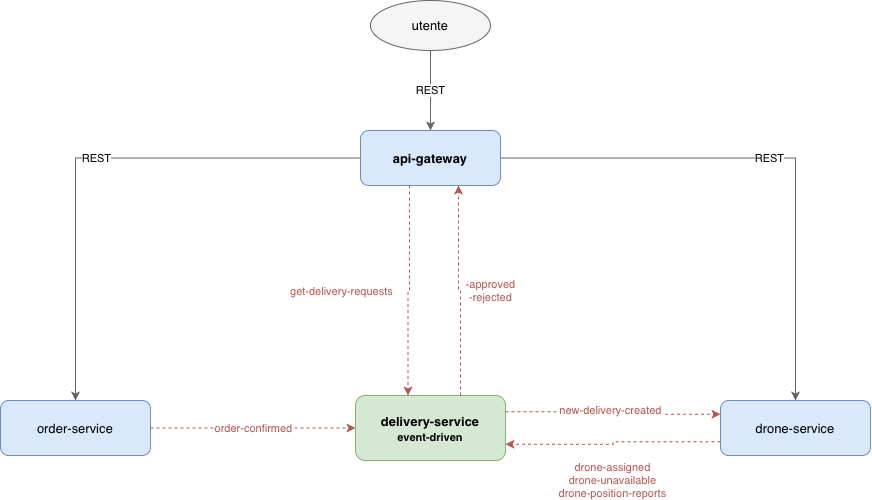
\includegraphics[width=\textwidth]{../doc/canali.png}
\caption{Canali di eventi e chiamate REST fra i servizi}
\label{fig:canali}
\end{figure}

\subsection{Comandi ed eventi}
\label{sec:dominio}

Non tutto ci\`o che viaggia sui canali ha la stessa natura, e la distinzione ha guidato la forma
degli adapter in uscita.

Un \textbf{comando} \`e rivolto a un destinatario preciso e attende un esito: chi lo invia decide
che cosa deve accadere. \`E il caso dell'interrogazione che l'api-gateway rivolge al
delivery-service per costruire il tracking, e infatti l\`i esiste una porta,
\texttt{DeliveryServicePort}, dichiarata dal livello applicativo del gateway e implementata da un
proxy.

Un \textbf{evento} constata un fatto avvenuto, non ha destinatario e non attende nulla: chi lo
riceve decide che cosa farne. \`E il caso dell'ordine confermato e della posizione di un drone.
Escono  attraverso gli \textbf{observer}, lo stesso meccanismo gi\`a usato dall'Assignment~2 per
l'osservabilit\`a, con una seconda implementazione che pubblica su un canale.

\begin{lstlisting}[caption={Il servizio annuncia, senza sapere chi ascolta}]
observers.forEach(o -> o.notifyOrderConfirmed(event));
\end{lstlisting}

Ne discende una propriet\`a verificabile del sistema: nell'intero progetto \textbf{esiste una sola porta}
verso il delivery-service, quella dell'api-gateway, ed esiste perch\'e il gateway \`e l'unico che
pone una domanda. Tutto il resto sono fatti annunciati.

Il beneficio pratico \`e che aggiungere un consumatore non costa nulla a chi pubblica: un servizio
interessato agli ordini confermati si iscrive al canale, e n\'e l'order-service n\'e il suo dominio
vengono toccati. Con un comando avremmo dovuto aggiungere una chiamata al mittente.

\paragraph{Rapporto con l'Event Sourcing.} Gli eventi che il dominio del delivery-service emette
restano \textbf{interni}: sono la sua fonte di verit\`a, vengono persistiti nell'event store e
alimentano il read model attraverso il proiettore.

\begin{lstlisting}[caption={Il read model e' derivato dallo stream, e ricostruibile da esso}]
newEvents.forEach(event -> projector.project(delivery.getId(), event));
\end{lstlisting}

Ci\`o che viaggia sui canali \`e invece un \textbf{evento di integrazione}: lo stesso fatto,
riformulato per chi lo riceve. L'evento di dominio \texttt{DeliveryScheduled} porta l'intera
\texttt{Route} e l'istante di creazione, perch\'e deve bastare a ricostruire l'aggregate nel replay;
l'annuncio \texttt{new-delivery-created} porta soltanto punto di ritiro e peso, che sono i due dati
su cui il drone-service decide se ha un mezzo adatto.

La distinzione \`e deliberata: pubblicare gli eventi di dominio cos\`i come sono renderebbe il
modello interno un \textbf{contratto pubblico}, e riorganizzare l'aggregate diventerebbe una
modifica da concordare con tutti i consumatori. I due rispondono del resto a criteri diversi: un
evento di dominio deve contenere quanto basta a \emph{ricostruire lo stato}, un evento di
integrazione quanto basta ad \emph{agire senza richiamare il mittente}.

% ============================================================
\section{Scaling e Service Levels}

\subsection{SLO e SLI}

Gli indicatori tipici con cui si esprime un livello di servizio sono disponibilit\`a, latenza,
tasso di errore, throughput e durabilit\`a. La scelta \`e caduta su \textbf{disponibilit\`a} e
\textbf{throughput}, i due che si agganciano agli scenari di qualit\`a gi\`a formulati
nell'Assignment~1: il primo alla continuit\`a del servizio in presenza di guasti, il secondo alla
scalabilit\`a sotto un volume crescente di ordini. Entrambi sono definiti sull'\textbf{api-gateway},
unico componente esposto all'esterno e quindi il punto di osservazione pi\`u vicino all'esperienza
d'uso.

\begin{table}[H]
\centering
\caption{Gli obiettivi e i rispettivi indicatori}
\begin{tabularx}{\textwidth}{lX}
\toprule
\textbf{SLO 1} & almeno il 99,5\% delle richieste servito con successo su 30 giorni \\
\textbf{SLI 1} & percentuale di richieste con status inferiore a 400 sul totale \\
\midrule
\textbf{SLO 2} & piu' di 40 richieste al secondo sostenute su 30 giorni \\
\textbf{SLI 2} & numero di richieste servite al secondo \\
\bottomrule
\end{tabularx}
\end{table}

Un 4xx \`e considerato un fallimento, perch\'e dal punto di vista dell'utente la richiesta non ha
prodotto quanto atteso. Le chiamate a \texttt{/health} sono invece \textbf{escluse} dal conteggio:
sono interrogazioni della piattaforma, ripetute a intervalli fissi e quasi sempre coronate da
successo, e includerle gonfierebbe l'indicatore con traffico che nessun utente ha generato.

L'obiettivo di throughput si aggancia allo scenario di scalabilit\`a dell'Assignment~1, che chiede
che un raddoppio del volume di ordini non produca degrado: dichiarare un livello sostenuto lo
trasforma da previsione in impegno verificabile.

\paragraph{Error budget.} Promettere il 99,5\% significa ammettere che lo 0,5\% pu\`o fallire. In
30~giorni ci sono 43.200~minuti, quindi quello 0,5\% vale \textbf{216~minuti}: circa tre ore e mezza
in cui il servizio pu\`o non funzionare senza aver mancato l'obiettivo.

\subsection{Strumentazione}

Entrambi gli indicatori si ricavano contando le richieste servite, distinguendo quelle riuscite dal
totale. Le metriche sono esposte dall'api-gateway sulla porta~9492.

\begin{table}[H]
\centering
\caption{Metriche introdotte nell'Assignment 3}
\begin{tabularx}{\textwidth}{llX}
\toprule
\textbf{Metrica} & \textbf{Tipo} & \textbf{Contenuto} \\
\midrule
\texttt{gateway\_requests\_total} & counter & richieste servite \\
\texttt{gateway\_successful\_requests\_total} & counter & quelle con status inferiore a 400 \\
\texttt{gateway\_response\_time\_seconds\_total} & counter & tempo di risposta accumulato \\
\bottomrule
\end{tabularx}
\end{table}

I primi due counter sono quanto serve agli indicatori: il loro rapporto \`e la disponibilit\`a, la
derivata del primo \`e il throughput. Il terzo non alimenta alcun obiettivo, ma diviso per il numero
di richieste fornisce il tempo medio di risposta, che resta un dato utile a osservare il sistema.

Nessuna metrica porta label. Si era valutato di distinguere le richieste per percorso, ma le rotte
contengono identificatori di risorsa, e usarli come valori di label farebbe crescere senza limite il
numero di serie temporali. La misura viene presa quando la risposta \`e stata scritta, unico momento
in cui sia lo status code sia la durata sono definitivi.

\begin{lstlisting}[caption={Le due query PromQL degli indicatori}]
sum(increase(gateway_successful_requests_total[30d]))
  / sum(increase(gateway_requests_total[30d]))

sum(rate(gateway_requests_total[30d]))
\end{lstlisting}

Il gateway \`e replicato, quindi entrambe le query sommano su tutte le istanze: i counter sono per
processo, e la somma li ricompone in un indicatore di sistema.

\subsection{Verifica degli indicatori}

Gli indicatori sono stati misurati sul deployment Kubernetes, sottoponendo il gateway a un carico
generato dall'interno del cluster da dodici client concorrenti, ciascuno dei quali ripete un ciclo
di due richieste valide e una destinata a fallire, per un totale di 8.100 richieste servite.

\begin{table}[H]
\centering
\caption{Valori osservati}
\begin{tabularx}{\textwidth}{lXl}
\toprule
\textbf{Indicatore} & \textbf{Atteso} & \textbf{Misurato} \\
\midrule
disponibilit\`a & 0,667, ossia due successi su tre & \textbf{0,6667} \\
throughput & superiore a 40~richieste al secondo & \textbf{138,5~req/s} \\
\bottomrule
\end{tabularx}
\end{table}

La coincidenza fra valore atteso e valore misurato per il primo indicatore \`e la verifica che la
metrica conteggia ci\`o che dichiara di conteggiare. Il secondo \`e il picco sostenuto durante la
prova, distribuito in modo uniforme sulle tre repliche, che hanno servito rispettivamente 2.733,
2.708 e 2.659 richieste.

Una prova precedente, condotta con un solo client sequenziale, aveva registrato un picco di appena
15,4~richieste al secondo. Il limite non era del sistema ma del generatore: un client che attende
ogni risposta prima di inviare la successiva non pu\`o produrre pi\`u richieste di quante ne
completi in sequenza.

Il protocollo di misura non \`e arbitrario: il \textbf{modello pull} di Prometheus impone tre
condizioni, in assenza delle quali l'indicatore restituisce un valore plausibile e falso.

\paragraph{Il carico deve durare pi\`u di un intervallo di scrape.} Prometheus non osserva le
richieste una per una: passa a intervalli regolari e legge il valore dei contatori. Se tutte le
richieste arrivano fra un passaggio e il successivo, alla prima lettura il contatore \`e gi\`a al
valore finale e da l\`i in poi non cresce pi\`u. La funzione \texttt{rate()}, che calcola di quanto
un contatore \`e cresciuto, non pu\`o usare quella prima lettura, perch\'e non sa da quale valore
partisse: vede solo la parte costante che segue e risponde zero, anche se nel frattempo erano
fallite decine di richieste.

\paragraph{Il carico va generato dall'interno del cluster.} Raggiungere il gateway da fuori con
\texttt{kubectl port-forward} sembra comodo, ma quel comando sceglie un pod all'inizio e continua a
usare sempre quello: tutte le richieste finirebbero su una replica sola, e le altre due
risulterebbero inattive. Inviando invece il carico dall'interno del cluster, all'indirizzo del
Service, il bilanciamento avviene davvero, come mostrano i conteggi quasi identici riportati
sopra.

\subsection{Deployment su Kubernetes}

Il sistema \`e descritto da sette manifest nella cartella \texttt{kubernetes/}: un namespace
dedicato, i quattro servizi, l'infrastruttura Kafka con Zookeeper, e Prometheus. Il cluster locale
utilizzato \`e \textbf{kind}. Poich\'e le immagini sono costruite localmente e non pubblicate su un
registry, vanno caricate nel nodo con \texttt{kind load docker-image} e i Deployment specificano
\texttt{imagePullPolicy: IfNotPresent}.

L'osservazione pi\`u rilevante riguarda ci\`o che \textbf{non} \`e stato necessario fare. Le
variabili d'ambiente dei manifest sono identiche a quelle del Docker Compose, perch\'e i servizi si
individuano per nome di Service e il DNS interno di Kubernetes li risolve esattamente come faceva
quello di Docker. Il pattern \textbf{Externalized Configuration}, adottato nell'Assignment~2, ha
quindi reso il passaggio di piattaforma possibile \textbf{senza modificare una riga di codice Java}.

Oltre a Deployment e Service, i manifest aggiungono due elementi non strettamente necessari a far
funzionare il sistema. Il primo sono le \textbf{probe} di liveness e readiness su tutti e quattro i
servizi, possibili senza scrivere codice perch\'e l'endpoint \texttt{/health} esisteva gi\`a
dall'Assignment~2. Il secondo \`e \textbf{Prometheus}, deployato nel cluster insieme ai servizi,
senza il quale gli indicatori sarebbero misurabili solo in esecuzione locale.

La distinzione fra le due probe merita di essere esplicitata, perch\'e agiscono su piani diversi: la
\emph{liveness} accerta che il processo sia vivo e in caso contrario lo sostituisce, mentre la
\emph{readiness} accerta che sia pronto a servire e in caso contrario lo rimuove dagli endpoint del
Service senza ucciderlo. Un servizio che sta ancora sottoscrivendo i propri canali \`e vivo ma non
pronto.

\subsection{Replicazione}

Il numero di repliche \`e portato a \textbf{tre solo per l'api-gateway}, che \`e l'unico componente
privo di stato proprio. Gli altri restano a una replica perch\'e il loro stato risiede in memoria:
con pi\`u repliche il drone-service assegnerebbe lo stesso drone a due consegne diverse. \`E il
limite gi\`a dichiarato nel report dell'Assignment~2, che il presente lavoro non rimuove ma
circoscrive.

Va precisato che cosa questa replicazione produce, per non attribuirle pi\`u di quanto dia. Produce
\textbf{disponibilit\`a}: la caduta di un'istanza non interrompe il servizio, come mostrato nella
sezione successiva. Non produce \textbf{throughput}, per tre ragioni concorrenti. Il collo di
bottiglia resta a valle, perch\'e ogni operazione di dominio converge su un delivery-service a
replica singola. Il canale di risposta \`e in broadcast, quindi il lavoro di lettura da Kafka viene
moltiplicato per il numero di repliche anzich\'e diviso. E ogni richiesta in volo trattiene un
thread fino alla risposta o al timeout. Aumentare la capacit\`a del sistema richiederebbe prima di
estrarre lo stato del delivery-service, poi di aumentare le partizioni dei suoi canali.

Replicare il gateway impone due vincoli che con una sola istanza non si porrebbero, e che hanno
determinato altrettante scelte di progetto.

\paragraph{Un consumer group per istanza, non per servizio.} All'interno di un gruppo ogni
partizione appartiene a un solo membro, e i canali di risposta ne hanno una soltanto: se le tre
repliche condividessero il gruppo \texttt{api-gateway}, tutte le risposte verrebbero recapitate a
una sola di esse e le altre due non ne riceverebbero alcuna. Poich\'e per\`o il Service distribuisce
le richieste in ingresso su tutte e tre, la replica che attende una risposta coincide con quella che
la riceve soltanto in un caso su tre: le altre due volte l'attesa si chiuderebbe in timeout.

La risposta a un \texttt{requestId} appartiene infatti alla replica che ne custodisce l'attesa in
memoria: il canale di risposta \`e un \textbf{broadcast}, non un carico da distribuire. Il gruppo
\`e quindi reso univoco per istanza, cos\`i che ogni replica riceva tutte le risposte e scarti
quelle non proprie. Gli altri tre servizi mantengono il gruppo fisso, che per essi \`e corretto
perch\'e le loro reazioni sono autosufficienti.

\begin{lstlisting}[caption={Un gruppo per istanza, non per servizio}]
static final String CONSUMER_GROUP = "api-gateway-" + UUID.randomUUID();
\end{lstlisting}

\paragraph{Un Service headless per lo scrape delle metriche.} Ogni replica tiene i propri contatori
in memoria, quindi i tre valori sono diversi fra loro. Un Service ordinario espone per\`o un solo
indirizzo e a ogni connessione ne sceglie una: Prometheus finirebbe per leggere ora l'una ora
l'altra, credendo di interrogare sempre la stessa sorgente. Il valore che registrerebbe salirebbe e
scenderebbe senza motivo apparente, e poich\'e un contatore che diminuisce viene interpretato come un
riavvio del processo, i tassi calcolati su quella serie sarebbero privi di senso.

Serve quindi che Prometheus veda i tre pod come tre sorgenti distinte. Lo si ottiene con un secondo
Service dichiarato \textbf{headless}, cio\`e privo di indirizzo proprio: il suo nome non corrisponde
a un punto d'ingresso unico, ma si risolve nell'elenco degli indirizzi di tutti i pod. Prometheus,
configurato per ricavare le proprie destinazioni da quella risoluzione, ne ottiene tre e le
interroga separatamente. La verifica sul cluster mostra \textbf{sei target attivi, di cui tre
distinti per il gateway}, uno per replica, e le query degli indicatori li ricompongono sommando.

Esiste un'alternativa in cui Prometheus interroga direttamente Kubernetes per farsi elencare i pod,
pi\`u generale perch\'e non richiede un Service dedicato, ma comporta l'introduzione di tre oggetti
di controllo degli accessi che il resto del sistema non usa.

\subsection{Self-healing osservato}

Il beneficio pi\`u immediato della piattaforma \`e il control loop che riporta lo stato osservato a
quello dichiarato. Eliminando manualmente un pod dell'api-gateway mentre il sistema era sotto
carico, il ReplicaSet ne ha creato immediatamente un altro, divenuto pronto in \textbf{45 secondi},
mentre le due repliche superstiti continuavano a servire senza interruzione: \`e la
disponibilit\`a che la replicazione promette, verificata invece che asserita.

Il broker \`e l'unico componente privo di probe, a differenza dei quattro servizi: non espone un
endpoint HTTP di salute, e i controlli di tipo \texttt{exec} disponibili si sono rivelati inadatti a
descriverne la disponibilit\`a. La sua indisponibilit\`a temporanea non blocca per\`o il sistema,
perch\'e i servizi che vi si collegano gestiscono da s\'e la riconnessione: la loro partenza non
dipende dall'ordine di avvio, come si \`e osservato durante le prove, quando un riavvio del broker
non ha richiesto di riavviare nulla d'altro.

A verifica conclusa, i pod applicativi hanno mantenuto lo stato pronto per \textbf{18~ore
consecutive senza alcun riavvio}.

% ============================================================
\section{Impatto sui test}

Il passaggio a un flusso non sincrono ha effetti diretti sulla verifica, perch\'e i test
dell'Assignment~2 asserivano immediatamente dopo l'azione, assumendo che al ritorno della chiamata
l'intera catena fosse conclusa. Tale assunzione non vale pi\`u per costruzione.

I test sono stati quindi riformulati in modo da \textbf{attendere che il sistema si assesti},
interrogando ripetutamente entro un budget di tempo anzich\'e verificare una sola volta. Lo scenario
end-to-end esprime ora questa attesa nel proprio testo, con la formulazione \emph{the delivery
eventually has a drone assigned}.

\`E stata inoltre introdotta la classe \texttt{BrokerAvailability}, che sospende i test dipendenti
dal middleware, tramite \texttt{Assumptions.abort()}, quando il broker non \`e raggiungibile: un test
che non pu\`o essere eseguito deve dichiararsi saltato e non fallito, altrimenti l'esito perde
significato.

% ============================================================
\section{Limiti noti}

\paragraph{Il delivery-service non \`e replicabile, e il motivo \`e duplice.} Event store, snapshot
e read model restano strutture dati in memoria, quindi due repliche avrebbero due verit\`a diverse.
A questo si aggiunge un secondo ostacolo, meno ovvio e specifico dell'architettura a eventi: i sette
canali in ingresso del servizio sono sottoscritti sotto un unico consumer group, per cui Kafka
distribuisce le loro partizioni \textbf{fra} le repliche invece di replicarne il consumo.

La cosa \`e stata verificata sul cluster portando il servizio a due repliche. L'assegnazione
osservata \`e stata la seguente:

\begin{lstlisting}[caption={Assegnazione dei canali con due repliche del delivery-service}]
pod A   order-confirmed, drone-unavailable
pod B   drone-assigned, drone-position-reports, get-delivery-requests
\end{lstlisting}

Il ciclo di vita di una singola consegna viene cos\`i spezzato fra due processi con memorie
separate: la consegna nasce in A, ma l'assegnazione del drone arriva in B, che non la conosce. Il
comportamento osservato \`e stato che nessuna consegna riceve pi\`u un drone e resta
indefinitamente in stato \texttt{SCHEDULED}, con il seguente messaggio nel log della replica B:

\begin{lstlisting}[caption={Esito osservato}]
WARNING: DroneAssigned discarded - Delivery not found: c5c7fdbe-565e-4e8a-b211-a6ff4d86508d
\end{lstlisting}

Va sottolineato che il guasto non \`e dovuto a Kafka, che si \`e comportato correttamente, n\'e
all'architettura a eventi: la stessa configurazione con lo stato in memoria si sarebbe rotta
identicamente nella versione sincrona dell'Assignment~2. Rendere il servizio replicabile richiede,
nell'ordine, uno store condiviso, un numero di partizioni maggiore di uno, e solo allora l'aumento
delle repliche.

\paragraph{Salvare gli eventi su file non basterebbe.} \`E l'evoluzione pi\`u immediata e
richiederebbe di sostituire un solo adapter, senza toccare il dominio, ma darebbe
\textbf{durabilit\`a e non replicabilit\`a}: due processi che scrivono lo stesso file non hanno modo
di coordinarsi, e il controllo di concorrenza oggi garantito all'interno di una sola macchina
virtuale verrebbe meno. Servirebbe uno store realmente condiviso, come un database, che imponga
esso stesso il controllo di versione. Su Kubernetes, inoltre, il file va montato su un volume
persistente, altrimenti sparisce a ogni riavvio del pod.

\paragraph{Uno stesso evento pu\`o essere elaborato due volte.} Elaborare un evento e registrare di
averlo fatto sono due operazioni distinte, e il segnalibro del consumatore avanza a intervalli
anzich\'e dopo ogni messaggio: un processo che termini fra le due riprende dall'evento che aveva
gi\`a elaborato. \`E la garanzia \emph{at-least-once}, e Kafka la preferisce all'alternativa, che
sarebbe perdere l'evento anzich\'e ripeterlo.

Gli handler dovrebbero quindi essere \textbf{idempotenti}, cio\`e produrre lo stesso risultato se
eseguiti una o pi\`u volte, e i nostri non lo sono: rileggere \texttt{order-confirmed} creerebbe una
seconda consegna per lo stesso ordine, e impegnerebbe un secondo drone. Sarebbe sufficiente
verificare l'esistenza di una consegna per quell'ordine prima di crearne una, interrogazione a cui
il read model sa gi\`a rispondere.

\paragraph{La finestra di 30 giorni non \`e osservabile.} Gli obiettivi sono enunciati su 30~giorni
perch\'e \`e la scala su cui un service level ha senso, ma il sistema viene avviato per la durata
delle prove e Prometheus non possiede quella storia. Le verifiche usano una finestra di pochi
minuti: cambia l'ampiezza del campione, non la forma dell'indicatore.

% ============================================================
\section{Conclusioni}

Sul piano della comunicazione, l'architettura a eventi ha sostituito l'\textbf{orchestrazione} con
la \textbf{coreografia}. Il risultato pi\`u sintetico \`e la firma del costruttore
dell'application service, passata da tre dipendenze a una: il delivery-service non conosce pi\`u
l'esistenza degli altri servizi e si limita a produrre fatti. Il prezzo \`e una consistenza
\emph{eventual}, che rende normale uno stato intermedio prima considerato degradato.

Sul piano operativo, i service level hanno reso continua una verifica che prima avveniva una volta
sola: gli scenari di qualit\`a si controllavano provocando una condizione, gli obiettivi si
osservano invece senza interruzione. Resta valido il principio enunciato nell'Assignment~2, \textbf{lo strumento di misura determina
quali attributi di qualit\`a \`e possibile promettere}: la latenza continua a non essere osservabile,
e finch\'e non lo sar\`a nessun obiettivo potr\`a essere formulato su di essa.

Le due direzioni si incontrano nel deployment. Replicare un componente ha fatto emergere due difetti
che con una sola istanza non si sarebbero mai visti, il consumer group condiviso e lo scrape
attraverso un servizio bilanciato: una scelta di deployment non \`e neutrale rispetto
all'architettura applicativa, ma ne verifica le assunzioni.

\end{document}
